\documentclass[10pt,conference]{IEEEtran}
% Some Computer Society conferences also require the compsoc mode option,
% but others use the standard conference format.
%
% If IEEEtran.cls has not been installed into the LaTeX system files,
% manually specify the path to it like:
% \documentclass[conference]{../sty/IEEEtran}

\usepackage[lined,boxed,commentsnumbered, ruled]{algorithm2e}
\usepackage{amsmath,epsfig,bm}
\usepackage{times}
\usepackage{array}
\usepackage{epigraph}
\usepackage{multirow}
\usepackage{caption}

%\newdef{intuition}{Intuition}
%\newdef{definition}{Definition}



% Some very useful LaTeX packages include:
% (uncomment the ones you want to load)


% *** MISC UTILITY PACKAGES ***
%
%\usepackage{ifpdf}
% Heiko Oberdiek's ifpdf.sty is very useful if you need conditional
% compilation based on whether the output is pdf or dvi.
% usage:
% \ifpdf
%   % pdf code
% \else
%   % dvi code
% \fi
% The latest version of ifpdf.sty can be obtained from:
% http://www.ctan.org/pkg/ifpdf
% Also, note that IEEEtran.cls V1.7 and later provides a builtin
% \ifCLASSINFOpdf conditional that works the same way.
% When switching from latex to pdflatex and vice-versa, the compiler may
% have to be run twice to clear warning/error messages.






% *** CITATION PACKAGES ***
%
%\usepackage{cite}
% cite.sty was written by Donald Arseneau
% V1.6 and later of IEEEtran pre-defines the format of the cite.sty package
% \cite{} output to follow that of the IEEE. Loading the cite package will
% result in citation numbers being automatically sorted and properly
% "compressed/ranged". e.g., [1], [9], [2], [7], [5], [6] without using
% cite.sty will become [1], [2], [5]--[7], [9] using cite.sty. cite.sty's
% \cite will automatically add leading space, if needed. Use cite.sty's
% noadjust option (cite.sty V3.8 and later) if you want to turn this off
% such as if a citation ever needs to be enclosed in parenthesis.
% cite.sty is already installed on most LaTeX systems. Be sure and use
% version 5.0 (2009-03-20) and later if using hyperref.sty.
% The latest version can be obtained at:
% http://www.ctan.org/pkg/cite
% The documentation is contained in the cite.sty file itself.






% *** GRAPHICS RELATED PACKAGES ***
%
\ifCLASSINFOpdf
  % \usepackage[pdftex]{graphicx}
  % declare the path(s) where your graphic files are
  % \graphicspath{{../pdf/}{../jpeg/}}
  % and their extensions so you won't have to specify these with
  % every instance of \includegraphics
  % \DeclareGraphicsExtensions{.pdf,.jpeg,.png}
\else
  % or other class option (dvipsone, dvipdf, if not using dvips). graphicx
  % will default to the driver specified in the system graphics.cfg if no
  % driver is specified.
  % \usepackage[dvips]{graphicx}
  % declare the path(s) where your graphic files are
  % \graphicspath{{../eps/}}
  % and their extensions so you won't have to specify these with
  % every instance of \includegraphics
  % \DeclareGraphicsExtensions{.eps}
\fi
% graphicx was written by David Carlisle and Sebastian Rahtz. It is
% required if you want graphics, photos, etc. graphicx.sty is already
% installed on most LaTeX systems. The latest version and documentation
% can be obtained at: 
% http://www.ctan.org/pkg/graphicx
% Another good source of documentation is "Using Imported Graphics in
% LaTeX2e" by Keith Reckdahl which can be found at:
% http://www.ctan.org/pkg/epslatex
%
% latex, and pdflatex in dvi mode, support graphics in encapsulated
% postscript (.eps) format. pdflatex in pdf mode supports graphics
% in .pdf, .jpeg, .png and .mps (metapost) formats. Users should ensure
% that all non-photo figures use a vector format (.eps, .pdf, .mps) and
% not a bitmapped formats (.jpeg, .png). The IEEE frowns on bitmapped formats
% which can result in "jaggedy"/blurry rendering of lines and letters as
% well as large increases in file sizes.
%
% You can find documentation about the pdfTeX application at:
% http://www.tug.org/applications/pdftex





% *** MATH PACKAGES ***
%
%\usepackage{amsmath}
% A popular package from the American Mathematical Society that provides
% many useful and powerful commands for dealing with mathematics.
%
% Note that the amsmath package sets \interdisplaylinepenalty to 10000
% thus preventing page breaks from occurring within multiline equations. Use:
%\interdisplaylinepenalty=2500
% after loading amsmath to restore such page breaks as IEEEtran.cls normally
% does. amsmath.sty is already installed on most LaTeX systems. The latest
% version and documentation can be obtained at:
% http://www.ctan.org/pkg/amsmath





% *** SPECIALIZED LIST PACKAGES ***
%
%\usepackage{algorithmic}
% algorithmic.sty was written by Peter Williams and Rogerio Brito.
% This package provides an algorithmic environment fo describing algorithms.
% You can use the algorithmic environment in-text or within a figure
% environment to provide for a floating algorithm. Do NOT use the algorithm
% floating environment provided by algorithm.sty (by the same authors) or
% algorithm2e.sty (by Christophe Fiorio) as the IEEE does not use dedicated
% algorithm float types and packages that provide these will not provide
% correct IEEE style captions. The latest version and documentation of
% algorithmic.sty can be obtained at:
% http://www.ctan.org/pkg/algorithms
% Also of interest may be the (relatively newer and more customizable)
% algorithmicx.sty package by Szasz Janos:
% http://www.ctan.org/pkg/algorithmicx




% *** ALIGNMENT PACKAGES ***
%
%\usepackage{array}
% Frank Mittelbach's and David Carlisle's array.sty patches and improves
% the standard LaTeX2e array and tabular environments to provide better
% appearance and additional user controls. As the default LaTeX2e table
% generation code is lacking to the point of almost being broken with
% respect to the quality of the end results, all users are strongly
% advised to use an enhanced (at the very least that provided by array.sty)
% set of table tools. array.sty is already installed on most systems. The
% latest version and documentation can be obtained at:
% http://www.ctan.org/pkg/array


% IEEEtran contains the IEEEeqnarray family of commands that can be used to
% generate multiline equations as well as matrices, tables, etc., of high
% quality.




% *** SUBFIGURE PACKAGES ***
%\ifCLASSOPTIONcompsoc
%  \usepackage[caption=false,font=normalsize,labelfont=sf,textfont=sf]{subfig}
%\else
%  \usepackage[caption=false,font=footnotesize]{subfig}
%\fi
% subfig.sty, written by Steven Douglas Cochran, is the modern replacement
% for subfigure.sty, the latter of which is no longer maintained and is
% incompatible with some LaTeX packages including fixltx2e. However,
% subfig.sty requires and automatically loads Axel Sommerfeldt's caption.sty
% which will override IEEEtran.cls' handling of captions and this will result
% in non-IEEE style figure/table captions. To prevent this problem, be sure
% and invoke subfig.sty's "caption=false" package option (available since
% subfig.sty version 1.3, 2005/06/28) as this is will preserve IEEEtran.cls
% handling of captions.
% Note that the Computer Society format requires a larger sans serif font
% than the serif footnote size font used in traditional IEEE formatting
% and thus the need to invoke different subfig.sty package options depending
% on whether compsoc mode has been enabled.
%
% The latest version and documentation of subfig.sty can be obtained at:
% http://www.ctan.org/pkg/subfig




% *** FLOAT PACKAGES ***
%
%\usepackage{fixltx2e}
% fixltx2e, the successor to the earlier fix2col.sty, was written by
% Frank Mittelbach and David Carlisle. This package corrects a few problems
% in the LaTeX2e kernel, the most notable of which is that in current
% LaTeX2e releases, the ordering of single and double column floats is not
% guaranteed to be preserved. Thus, an unpatched LaTeX2e can allow a
% single column figure to be placed prior to an earlier double column
% figure.
% Be aware that LaTeX2e kernels dated 2015 and later have fixltx2e.sty's
% corrections already built into the system in which case a warning will
% be issued if an attempt is made to load fixltx2e.sty as it is no longer
% needed.
% The latest version and documentation can be found at:
% http://www.ctan.org/pkg/fixltx2e


%\usepackage{stfloats}
% stfloats.sty was written by Sigitas Tolusis. This package gives LaTeX2e
% the ability to do double column floats at the bottom of the page as well
% as the top. (e.g., "\begin{figure*}[!b]" is not normally possible in
% LaTeX2e). It also provides a command:
%\fnbelowfloat
% to enable the placement of footnotes below bottom floats (the standard
% LaTeX2e kernel puts them above bottom floats). This is an invasive package
% which rewrites many portions of the LaTeX2e float routines. It may not work
% with other packages that modify the LaTeX2e float routines. The latest
% version and documentation can be obtained at:
% http://www.ctan.org/pkg/stfloats
% Do not use the stfloats baselinefloat ability as the IEEE does not allow
% \baselineskip to stretch. Authors submitting work to the IEEE should note
% that the IEEE rarely uses double column equations and that authors should try
% to avoid such use. Do not be tempted to use the cuted.sty or midfloat.sty
% packages (also by Sigitas Tolusis) as the IEEE does not format its papers in
% such ways.
% Do not attempt to use stfloats with fixltx2e as they are incompatible.
% Instead, use Morten Hogholm'a dblfloatfix which combines the features
% of both fixltx2e and stfloats:
%
% \usepackage{dblfloatfix}
% The latest version can be found at:
% http://www.ctan.org/pkg/dblfloatfix




% *** PDF, URL AND HYPERLINK PACKAGES ***
%
%\usepackage{url}
% url.sty was written by Donald Arseneau. It provides better support for
% handling and breaking URLs. url.sty is already installed on most LaTeX
% systems. The latest version and documentation can be obtained at:
% http://www.ctan.org/pkg/url
% Basically, \url{my_url_here}.




% *** Do not adjust lengths that control margins, column widths, etc. ***
% *** Do not use packages that alter fonts (such as pslatex).         ***
% There should be no need to do such things with IEEEtran.cls V1.6 and later.
% (Unless specifically asked to do so by the journal or conference you plan
% to submit to, of course. )


% correct bad hyphenation here
\hyphenation{op-tical net-works semi-conduc-tor}


\begin{document}
%
% paper title
% Titles are generally capitalized except for words such as a, an, and, as,
% at, but, by, for, in, nor, of, on, or, the, to and up, which are usually
% not capitalized unless they are the first or last word of the title.
% Linebreaks \\ can be used within to get better formatting as desired.
% Do not put math or special symbols in the title.
\title{S-CAT: Summarization for Crowdsourced Android Testing}


% author names and affiliations
% use a multiple column layout for up to three different
% affiliations
\author{\IEEEauthorblockN{1st Author}
\IEEEauthorblockA{School of Electrical and\\Computer Engineering\\
Georgia Institute of Technology\\
Atlanta, Georgia 30332--0250\\
Email: http://www.michaelshell.org/contact.html}
\and
\IEEEauthorblockN{2nd Author}
\IEEEauthorblockA{Twentieth Century Fox\\
Springfield, USA\\
Email: homer@thesimpsons.com}
\and
\IEEEauthorblockN{3rd Author}
\IEEEauthorblockA{Starfleet Academy\\
San Francisco, California 96678--2391\\
Telephone: (800) 555--1212\\
Fax: (888) 555--1212}}

% conference papers do not typically use \thanks and this command
% is locked out in conference mode. If really needed, such as for
% the acknowledgment of grants, issue a \IEEEoverridecommandlockouts
% after \documentclass

% for over three affiliations, or if they all won't fit within the width
% of the page, use this alternative format:
% 
%\author{\IEEEauthorblockN{Michael Shell\IEEEauthorrefmark{1},
%Homer Simpson\IEEEauthorrefmark{2},
%James Kirk\IEEEauthorrefmark{3}, 
%Montgomery Scott\IEEEauthorrefmark{3} and
%Eldon Tyrell\IEEEauthorrefmark{4}}
%\IEEEauthorblockA{\IEEEauthorrefmark{1}School of Electrical and Computer Engineering\\
%Georgia Institute of Technology,
%Atlanta, Georgia 30332--0250\\ Email: see http://www.michaelshell.org/contact.html}
%\IEEEauthorblockA{\IEEEauthorrefmark{2}Twentieth Century Fox, Springfield, USA\\
%Email: homer@thesimpsons.com}
%\IEEEauthorblockA{\IEEEauthorrefmark{3}Starfleet Academy, San Francisco, California 96678-2391\\
%Telephone: (800) 555--1212, Fax: (888) 555--1212}
%\IEEEauthorblockA{\IEEEauthorrefmark{4}Tyrell Inc., 123 Replicant Street, Los Angeles, California 90210--4321}}




% use for special paper notices
%\IEEEspecialpapernotice{(Invited Paper)}




% make the title area
\maketitle

% As a general rule, do not put math, special symbols or citations
% in the abstract
\begin{abstract}
Testing a new Android application is hard, since the android platform has a lot of portability and
compatibility issues. These issues are caused by its fragmentation and
diversified operating-system versions, as well as varied hardware platforms, which can hardly be addressed. Due to this fact,
crowdsourcing emerged as an ideal way to perform the android testing, as workers
possess devices that could cover a large amount of both the operation-system versions and the hardware platforms.
Additionally, the diversified network settings of crowdsourced workers contribute to this task.
However, the manual reporting process can be cumbersome and still need some professional background, which dampens the
enthusiasm of the workers. In this paper, we propose a framework to \textbf{S}ummarize the \textbf{C}rowdsourced
\textbf{A}ndroid \textbf{T}esting (\emph{S-CAT}), which endeavours to ease the workload
of workers during the process of crowdsourcing. Specifically, we extract activities from workers and bug patterns
from a generated event sequence, and develop a \emph{T}esting \emph{P}rocess \emph{D}escription (\emph{TPD}) system
to produce a textual recounting based on the extracted information. We also propose possible experimental designs
to evaluate the efficacy of \emph{S-CAT}, and present results of a pilot evaluation of our initial framework.
Our results demonstrate that \emph{S-CAT} can both effectively improves the efficiency of workers and facilitates
debugging.
\end{abstract}

% no keywords




% For peer review papers, you can put extra information on the cover
% page as needed:
% \ifCLASSOPTIONpeerreview
% \begin{center} \bfseries EDICS Category: 3-BBND \end{center}
% \fi
%
% For peerreview papers, this IEEEtran command inserts a page break and
% creates the second title. It will be ignored for other modes.
\IEEEpeerreviewmaketitle



\section{Introduction}
Recent years have witnessed explosive increase of adoption of mobile computing, which is
almost ubiquitous with over $2.7$ billion active mobile users according to a survey in $2014$ \cite{ericsson2014ericsson}.
In the meantime, an increased demand for high-quality, robust mobile applications is being driven by this
growing user base that performs a series of computing tasks on ``smart'' devices, including daily news alert services,
traffic services, restaurant and entertainment listings, and mobile commerce applications.
Software testing is known to be generally expensive \cite{tassey2002economic}.
And mobile application testing can be more challenging due to some unique hardware and software features of mobile devices, 
e.g., mobile context, connectivity, small screen size, and restrictive data entry methods \cite{zhang2005challenges}.
\emph{Mobile context} typically includes the location, identities of nearby people, objects, as well as environmental elements.
\emph{Connectivity} issue is about the various network conditions that shall be taken into consideration in mobile application testing \cite{longoria2001designing}. Due to the
physical constraints of mobile devices, especially the \emph{small screen size}, some direct presentation of web pages
in mobile applications can be aesthetically unpleasant and even illegible \cite{bickmore1997digestor}.
Small buttons and labels limit users' effectiveness and efficiency in entering data, which may reduce the input speed
and increase errors, thus the \emph{restrictive data entry methods} is another critical issue in mobile application testing.

\begin{figure*}[!htbp]
\centering
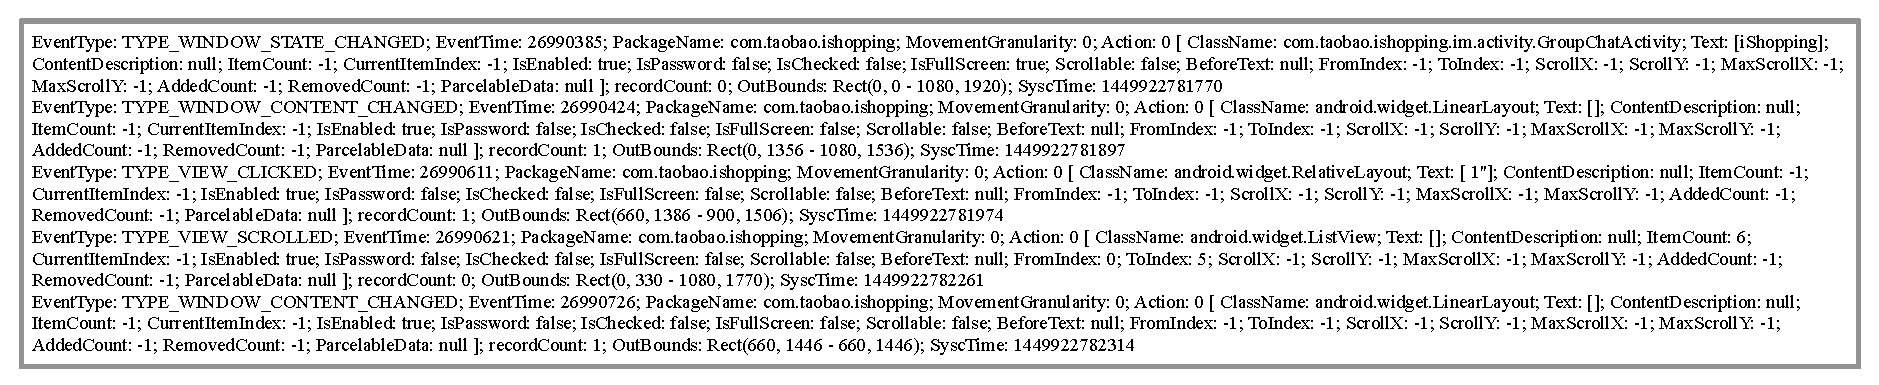
\includegraphics[width=2\columnwidth]{Figure/eventSample.eps}
\caption{An example of the event sequence}
\label{eventSample}
\end{figure*}


Currently, most mobile application testing is conducted through controlled laboratory experiments, i.e., human participants
are required to accomplish specific tasks in a controlled laboratory setting. However, this testing manner may miss the testing
of mobile context feature or other features we mentioned above. In addition to that, many mobile applications are developed by individual
developer, who lacks resources of performing software testing.

Crowdsourcing refers to outsourcing works, which are traditionally performed by an employee, to an ``undefined, generally large group
of people in the form of an open call'' \cite{vander2009crowdsourcing}. It is based on a simple but powerful concept:
Virtually anyone has the potential to plug in valuable information. To this point, it's natural for us to turn to crowdsourcing in performing
the mobile application testing, considering all the unique features mentioned above. As groups are under various network
conditions, possessing varied brands of mobile devices, using different versions of operating system releases. 

However, we meet several challenges when launching  the Crowdsourcing task. The first challenge is,
the accuracy of data isn't unfounded, but it's impossible to vet everyone, and to restrict who posts data online defeats
the entire purpose of crowdsourcing. For another, publicizing a crowdsourcing platform and establish a network of volunteers
can be extremely challenging \cite{greengard2011following}. In a word, how to measure and manage quality in crowdsourcing
systems has become an open problem. Currently, there are mainly two sets of approaches that aim at the quality control in crowdsourcing \cite{allahbakhsh2013quality},
i.e., the design-time approaches, e.g., effective task preparation and worker selection \cite{dow2012shepherding, kittur2008crowdsourcing, quinn2011human},
and the other is  runtime approaches, e.g., expert review, ground truth, majority consensus, contributor evaluation, real-time
support and workflow management \cite{dow2012shepherding, kittur2011crowdforge, kulkarni2012collaboratively}.

Android is the dominant mobile application platform, and in our initial work we mainly focus on the android testing.
In our implementation of crowdsourced android testing, we developed the Kikbug\footnote{http://kikbug.net} platform.
The working process is as follows, a requester first publishes a testing job, and workers take the job and submit the testing results before the
deadline. However, during our initial deployment, we find an critical issue, which is, the workers have to manually write the bug report,
for those that are not professionals, it could be complicated, also, to type in the textual description through mobile devices is somehow
inconvenient, which dampens workers' enthusiasm. So we are wondering how to adopt the runtime approaches to aid the workers,
and we come up with the idea of real-time support, that is, we summarize the event sequence of a worker, and then auto-generate the bug report.

\emph{AccessibilityServices} is an Android framework to provide alternative navigation feedback to the user on behalf of
applications installed on Android devices. Our tool takes advantage of such service to capture the working process of workers.
Figure \ref{eventSample} shows a worker's snipped testing process. Obviously, it is not easy for humans to get intuitive view of
the worker's testing processing, in terms of expressiveness and data volume. So we seek to reduce such volume, and turn to summarization.
In our vision, a good textual summary of such testing process will, on one hand, ease the workers' workload, on the other hand, help the developer obtain the maximal information from the
testing result of a worker, without having to inspect through the whole event sequence. A single summary could for example describe
a bunch of similar testing process of different workers, or a summary could describe why a specific testing process leads to the reproduction
of a certain bug. When performing crowdsourced mobile application testing, such summary can also enhance workers' experience,
as they no longer have to write the bug report themselves.
 

The problem we target in this paper is that manually reporting during the crowdsourced android testing is cumbersome
and may need some professional background, which dampens the enthusiasm of the workers.
Given a bunch of evidence from various modalities collected through our Kikbug tool, including system exchange information, event sequence
and screenshots, we summarize the testing results of a worker. Specifically, the \emph{S-CAT} system first learns a classification model which
decides whether a worker finds bug or not, and then it chooses the modules that are potentially bugs-related, thirdly, the system picks out the
snippets of event sequence which are most probably leading to the reproduction of the bugs, lastly, a Template-based Testing Process Description (\emph{TPD})
system produces recounting passages for the crowdsourced worker, in the format of natural language. A topic-independent planner module creates the
summary by suitably concatenating the output of multiple, specialized \emph{TPD} modules, which use a unique, manually written
natural language template, respectively, to generate a sentence about event sequence, and its importance.


\begin{figure}[!t]
\centering
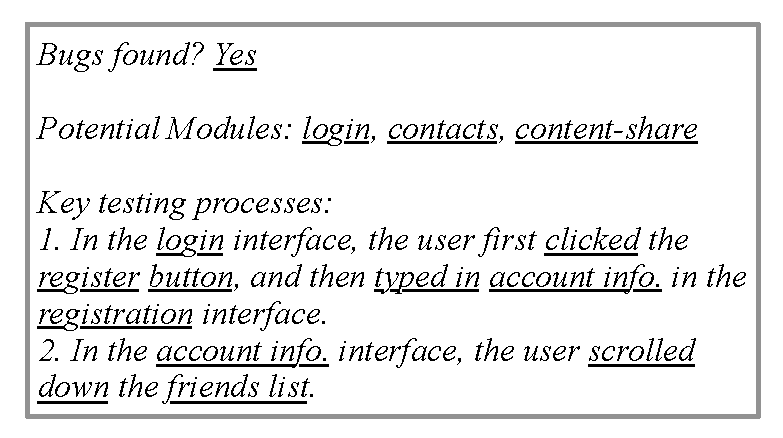
\includegraphics[width=0.73\columnwidth]{Figure/SummarySample}
\caption{An example of summarization}
\label{fig:sumsample}
\end{figure}

To sum up, our paper makes the following major contributions:

\begin{itemize}
\item We identify the challenges in mobile application testing, as well as the challenges in crowdsourcing. And come up with the idea
to summarize the crowdsourced android testing, as a means of real-time support in crowdsourcing. 
\item We propose the \emph{S-CAT} framework to tackle several challenges of our proposals including validating the testing process, module
probability, event sequence selection, and describing the testing process.
\item We conduct an extensive set of experiments based on $3$ real-world android applications, and the results empirically
demonstrated that the generated summary both facilitate the workers of working experience and the developers in debugging.
\end{itemize}

The reminder of this paper is organized as follows. Section \ref{problemDef} introduces the preliminary concepts and the problem statement.
The \emph{S-CAT} framework is presented in Section \ref{s-cam}. Section \ref{evaluation} presents the design of evaluation approaches,
as well as the metrics adopted. The experimental results are described in Section \ref{exp}, along with the discussion. Related work is presented in
Section \ref{relatedwork}. Section \ref{conclusions} concludes this article.


\section{Problem Statement}\label{problemDef}

In this section, we introduce some preliminary concepts, and formally define the problem of summarization for crowdsourced android
testing. Table \ref{tb:notations} summarizes the major notations used in the rest of the paper.

\begin{table}[!h]
\small
\centering
\caption{Notations used in the paper}
\begin{tabular}{c|c}
\hline
 SYMBOL&   DEFINITION\\\hline
    $u$ & crowdsourced worker \\\hline
    $p$ & android application\\\hline
$W^{u}_p$ & working profile related to $u$, $p$\\\hline
$l^{u}_p$ & logcat file related to $u$, $p$\\\hline
$e^{u}_p$ & event sequence related to $u$, $p$\\\hline
$s^{u}_p$ & screenshots related to $u$, $p$\\\hline
$d^{u}_p$ & device info. related to $u$, $p$\\\hline
    $a^{u}_p$ & $u$'s activities representation of application $p$\\\hline
    $a^{u}_p[i]$ & $i$th activity of $a^{u}_p$ \\\hline
    $K$ &  the length of event sequence\\\hline
    $L$ &  the number of attributes\\\hline
    $N$ &  the number of activities\\\hline
\end{tabular}
\label{tb:notations}
\end{table}


\subsection{Preliminary Concepts}

\newtheorem{definition}{Definition}
\begin{definition}
\emph{(Working Profile)}
For worker $u$'s testing process on application $p$,  we create a working profile $W^{u}_p$,
which is a set of  various modalities associated with $p$ and $u$,
collected via our Kikbug crowdsourcing client.
\end{definition}

Normally, the raw working profiles
consist of four aspects, however, in the real-world crowdsourced testing scenario, we observe that,
the event sequence is not directly usable for summarization purpose, due to the following four reasons: (1) There are many
redundant snippets of event sequences, which cause the data volume to be huge. (2) Many snippets are
meaningless, resulted by meaningless actions of workers, e.g., starting an application and exiting an application.
(3) For some certain events, there are attributes that are meaningless. (4) We notice that for some working profile,
there are certain attributes with null value throughout the event sequence.

Therefore, in our framework, we preprocess the raw working profiles in order to make them applicable.
Firstly, we remove the meaningless snippets that correspond to meaningless actions
of workers. (2) Then we remove the meaningless attributes attached to certain events, for example, the attribute
\emph{ispassword} is meaningless for most events. (3) Lastly, we remove the attributes that have null value throughout
the event sequence in a working profile. Details of the techniques of preprocessing raw working profiles are
described in Section \ref{s-cam}.


\begin{definition}\label{def:logcat}
 \emph{(Logcat)}
A logcat $l^{u}_p$ collects the system debug output, such as stack traces when an error is thrown and
messages generated by the android \emph{log} class.
\end{definition}

\begin{definition}
 \emph{(Event Sequence)}
An event sequence $e^{u}_p$ is information obtained through the android \emph{AccessibilityService}\footnote{http://developer.android.com/guide/topics/ui/\\accessibility/index.html}
during the working process of a testing job. It contains the UI event type, class name of the object in which the event occurred or originated, and string
value representing some associated data.
\end{definition}

\begin{definition}
 \emph{(Device Inoformation)}
Device information $d^{u}_p$ represents the running environment of the android application, including the brand of the device, the screen size, the
resolution, the android system version, as well as the release.
\end{definition}

\begin{figure}[!htbp]
\centering
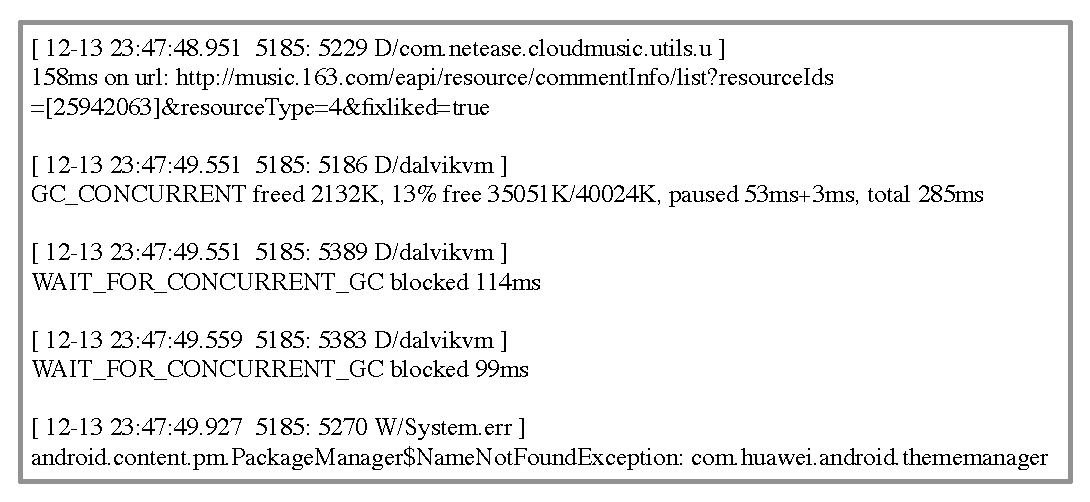
\includegraphics[width=0.85\columnwidth]{Figure/logcat}
\caption{An example of logcat}
\label{fig:logcat}
\end{figure}

Figure \ref{fig:logcat} shows an example of the logcat. Every record is in the $(time, processID, threadID, priority/tag, message)$ format,
where the priority is one of the following character values, ordered from lowest to highest:
\emph{V - Verbose (lowest priority)}, \emph{D - Debug}, \emph{I - Info}, \emph{W - Warning}, \emph{E - Error}, \emph{F - Fatal}, \emph{S - Silent (highest priority)}.


Figure \ref{eventSample} demonstrates an example of a snippet of an event sequence.
Each record represents an event, e.g., the first record stands for an event that relates to the state changing of a window type.
Naturally, the receipt of an event and its associated data and its
ability of querying window content present a security risk, and to mitigate this risk, in our implementation we require that \emph{AccessibilityServices}
enabled manually by the user and displays a dialog window alerting the user to the risk.

Notably, in our scenario of summarization, we may not use all the above information, but in order to best illustrate the workflow and specify
the files generated along our crowdsourced android testing, we introduce all these concepts.


\subsection{Problem Definition}

In adoption of the concept ``real-time support'' in runtime approaches that aim at quality control in crowdsourcing \cite{allahbakhsh2013quality},
we come up with the idea of summarization in our specified scenario, i.e., the crowdsourced android testing. Ideally, a good bug report
of a user shall contain
components such as whether a bug is detected or not, the module which the bug is related, as well as the scene in which the bug can be
reproduced, in the meantime, the testing environment like the hardware and operating system could be included as well.
We formulate our problem as follows:

\begin{figure*}[!htbp]
\centering
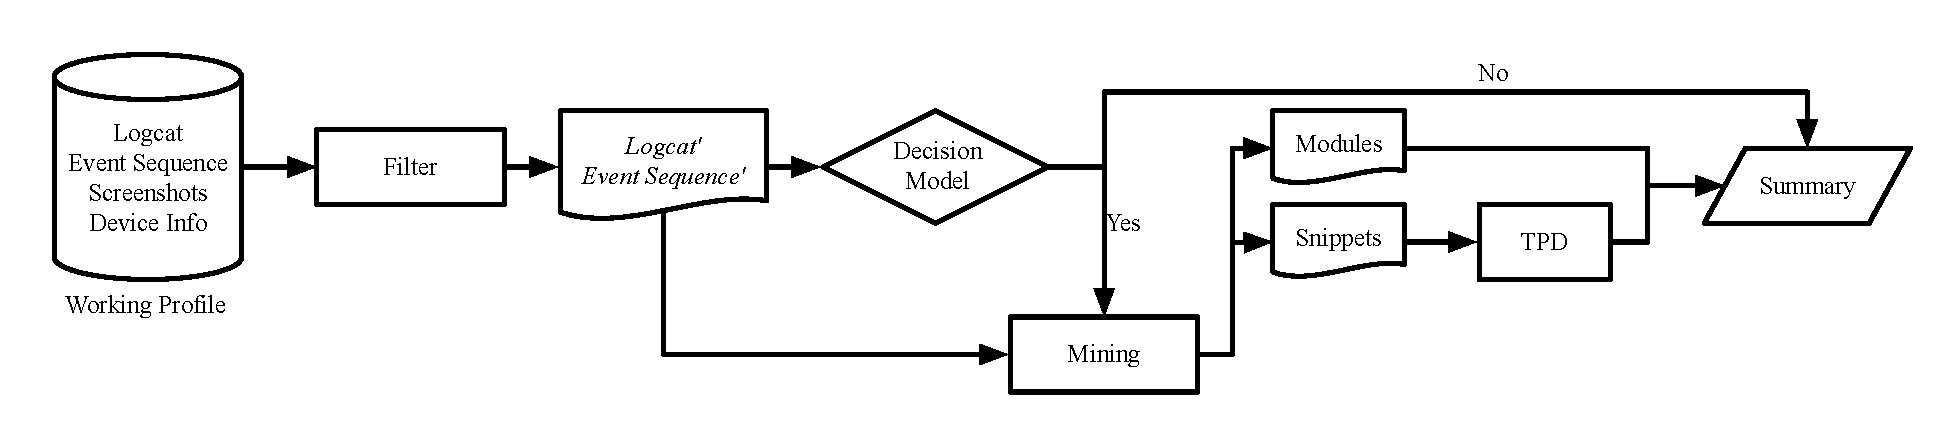
\includegraphics[width=1.8\columnwidth]{Figure/scam.eps}
\caption{Overview of \emph{S-CAT}}
\label{fig:scam}
\end{figure*}

\newtheorem{problem}{Problem}
\begin{problem} \textbf{(Summarization of Crowdsourced Android Testing)}
Given a working profile $W^{u}_p$, our goal is to summarize the working process of worker in android testing.
The output consists of three components, 1) whether bugs are found or not by the crowdsourced worker. 2) the modules that
are potentially bugs-related. 3) the event sequence snippet that probably reproduces the bug. And this information is presented as
well structured English readable sentences.
\end{problem}

\section{The S-CAT}\label{s-cam}

This section describes the details of the \emph{S-CAT} framework.
Generally speaking, our approach creates a summary of the working process of a crowdsourced worker performing
the android  application testing. And the workflow of \emph{S-CAT} corresponds to four major phases, as will be described
in the following. The architecture of our approach is shown in Figure \ref{fig:scam}. 

\subsection{Preprocess Phase}

The \emph{Preprocess Phase} corresponds to the filtering component in the \emph{S-CAT} architecture, which deals
with the working profile. The output of this phase is the filtered \emph{Logcat'} and \emph{Event Sequence'}.

\subsubsection{Logcat Filtering}
We take advantage of the android logging system which provides the mechanism for collecting and viewing system debug
output. Logs from various applications and portions of the system are collected to form the logcat file.
And $(time, processID, threadID,\\priority/tag, message)$ is the style our customized logcat file follows,
as shown in the example in Figure \ref{fig:logcat}. However, the collected logcat file is large in volume, which
is beyond manageable. Our goal of logcat filtering is to remove the irrelevant records which is on the kernel-level,
while retain the mobile application related ones.

As mentioned in \emph{Definition} \ref{def:logcat}, each log message has a \textit{tag} and a \textit{priority} associated with
it.  The \textit{tag} is a short string indicating the module/component from which the message originates, and the \textit{priority} that indicates different levels. 
We define a screenshot event
in the \texttt{Debug} priority, which saves the screen when the worker think he/she finds a bug (but this is optional for the worker).
In our initial trial of summarization, we only use the logcat file as labels, that is, we use the timestamp to locate 
certain activities from the event sequence, e.g., \texttt{Debug}, \texttt{Warning}
and \texttt{Error}, as to identify the high risk modules or components that are potentially
bugs-related. And in the meantime, we use these timestamps as evidences to extract the event sequence snippets that might
reproduce the bugs. In detail, we retain log messages with the following three priorities, which is \texttt{Debug}, \texttt{Warning}
and \texttt{Error}, and remove others.

\subsubsection{Event Sequence Filtering}
The goal of event sequence filtering is to filter out the noisy contents such as meaningless attributes and redundant snippets.
Android provides a \texttt{Java API} to its accessibility framework to enable developers integrate accessibility functionality into
customized applications. All drawable elements derive from a common ancestor, the View class, which contains built-in calls
to \emph{Accessibility} API methods. And in that way, most user interface widgets in the Android framework make their accessibility
information available, such as the UI event type, class name of the object in which the event occurred or originated, and string value
representing the associated data could be populated into an \emph{AccessibilityEvent} object and dispatched to enabled
\emph{AccessibilityServices} via the appropriate method call. Totally, there are $25$ \emph{AccessibilityEvent}
types\footnote{http://developer.android.com/reference/android/view/\\accessibility/AccessibilityEvent.html}.

Our collected event sequence (\emph{AccessibilityEvent}) covers almost all the above types of events, and
is formed of the attributes as shown in Table \ref{tab:eventSequence}.

\begin{table}[!htbp]
\centering
\tiny
\caption{Attributes of Events}
\begin{tabular}{c|c} \hline
ATTRIBUTE &DESCRIPTION\\ \hline
EventType & event type\\ \hline
EventTime & time when the event was sent\\ \hline
PackageName & package name of the source\\ \hline
MovementGranularity & movement granularity that was traversed\\ \hline
Action & action performed on an AccessibilityNode\\ \hline
ClassName & class name of the source\\ \hline
Text & text of the event\\ \hline
ContentDescription & description of the source\\ \hline
ItemCount & number of items that can be visited\\ \hline
CurrentItemIndex & index of the source can be visited\\ \hline
IsEnabled & if the source is enabled\\ \hline
IsPassword & if the source is a password field\\ \hline
IsChecked & if the source is checked\\ \hline
IsFullScreen & if the source is taking the entire screen\\ \hline
Scrollable & if the source is scrollable\\ \hline
BeforeText & the text before a change\\ \hline
FromIndex & the beginning of a text selection \\ \hline
ToIndex &  index of text selection \\ \hline
ScrollX &   the scroll offset of the source left edge \\ \hline
ScrollY &   the scroll offset of the source top edge \\ \hline
MaxScrollX &  the max scroll offset of the source left edge\\ \hline
MaxScrollY &  the max scroll offset of the source top edge\\ \hline
AddedCount &  the number of added characters \\ \hline
RemovedCount &  the number of removed characters \\ \hline
ParcelableData &  the Parcelable data\\ \hline
recordCount &  the number of records contained in the event \\ \hline
OutBounds & bounding rectangle\\ \hline
\end{tabular}
\label{tab:eventSequence}
\end{table}

Besides the problem of large volume, there are following issues that concerns the direct use
of the event sequence file by our careful analysis of the event sequence.
\begin{itemize}
\item \emph{Meaningless snippets.} By meaningless snippets we mean the meaningless \emph{Activities}. An
\emph{activity} is an application component that provides a screen with which the workers can interact with. Each activity consists of a group of events.
An event is generated when user interacts with the android system, such as dialling the phone, taking a snapshot, viewing a map.
But not all events are related to main business logic of the applications.

\item \emph{Redundant snippets.} Workers may wander around some specific interface of an application, which
generates a large amount of duplicate activities.

\item \emph{Meaningless attributes throughout the working profile.} For a specific application, there might be some attributes
that have \emph{Default} value throughout the working profile, which means this application doesn't interfere with certain attributes
during the functioning procedure.

\item \emph{Meaningless attributes for specified event type.} For certain types of event, there are some attributes that just do
no count at all, this is easy to understand, for example, for the event \emph{TYPE\_WINDOWS\_CHANGED}, the attribute field
\emph{IsPassword} just doesn't mean anything.
\end{itemize}

\begin{algorithm}[!htbp]
\small
\caption{Remove Redundant Snippets}
\label{alg:redundant}
\BlankLine
\LinesNumbered
\KwIn{Event Sequence $e^{u}_p$ of a Working Profile $W^{u}_p$;}
\KwOut{Event Sequence $e'^{u}_p$;}
Transform the $e^{u}_p$ into $a^{u}_p$;\\
$a'^{u}_p$ = ``'';\\
preA = $a^{u}_p[0]$;\\
\For{$i$ from $1$ to $N$} {
\If {$a^{u}_p[i]$ != preA}
{$a'^{u}_p$ += $a^{u}_p[i]$;}
preA = $a^{u}_p[i]$;
}
Transform the $a'^{u}_p$ into $e'^{u}_p$.\\
\end{algorithm}


\begin{algorithm}[!htbp]
\small
\caption{Remove Meaningless Attributes}
\label{alg:attributes}
\BlankLine
\LinesNumbered
\KwIn{Event Sequence $e^{u}_p$ of a Working Profile $W^{u}_p$;}
\KwOut{Event Sequence $e'^{u}_p$;}
Represent $e^{u}_p$ as Matrix $M(K,L)$;\\
Reverse Matrix $M(K,L)$ into Matrix $M'(L,K)$;\\
\For{$i$ from $1$ to $L$} {
\If {row i contains the same value}
{remove row $i$;}
}
Obtain the new Matrix Matrix $M'(L',K)$;\\
Reverse Matrix $M'(L',K)$ into Matrix $M'(K,L')$;\\
Generate $e'^{u}_p$ from Matrix $M'(K,L')$.\\
\end{algorithm}


Following above four issues, we perform the event sequence filtering. In detail, 
1) for \emph{Meaningless snippets}, we dig out some common activities from a wide range of different working profiles using the sequential
patterns mining tool \cite{fournier2014fast}, thus to get the common activities among the android applications, which are not application-specific. 
2) for \emph{Redundant snippets}, the goal of this step is to identify and remove the continual duplicate activities, which is application-dependent.
In our implementation, for continual duplicate activities we only retain a single one, the method is presented in Algorithm \ref{alg:redundant}.
3) for \emph{Meaningless attributes throughout the working profile}, the processing method is shown in Algorithm \ref{alg:attributes}. 
4) for \emph{Meaningless attributes for specified event type}, we discussed with the android developers from industry to manually recognize
the attributes that are of no use to certain types of events, and finally obtain the simplified format for each type of events.


\subsection{Decision Model}\label{decision}

The result of this component in the framework corresponds to the first part of the final summary, which tells whether
bugs are found or not by the worker. Intuitively, by identifying a set of various activities and interactions with systems of workers,
we can tell if the worker finds bugs or not in most cases. And follow this intuition, we pick out some of these activities as features that can
be used to train a classifier for further usage. In the initial implementation of this component of \emph{S-CAT}, we only use the following
four features to train the classification model, which generates an acceptable result by our study. In fact, it is an open question
of how to choose suitable features as to effectively train a classifier, as well as choosing which classification algorithm.  
That is, our framework is extensible in this sense. In this study, we adopt the LIBSVM \cite{chang2011libsvm} tool for the implementation.

\emph{The number of screenshots.} Intuitively, in the design of mechanism of our crowdsourced android testing,
we encourage the workers submit screenshots when they think they find a bug, thus to provide sufficient evidence for developers
in debugging. In this sense, we conclude the numbers of screenshots as a strong feature of the finding of bugs.

\emph{Pause time.} Based on our observation, when performing the crowdsourced testing, the workers would stop for a while
when they think they find a bug, and this will result in the abnormal time slot between the events, in fact, this phenomenon follows
the cognitive psychology, as a decision will always take some mental computing. Following this, we adopt the pause time as another
important feature in deciding the finding of bugs. By the way, here we use a threshold in defining the \emph{Pause}. 

\emph{Time compared to other workers.} This feature is intended to distinguish the consuming time of workers in conducting a
crowdsourcing task, the hypothesis behind it is quite simple, when a worker spends time more than the average time of other
workers on a certain crowdsourced android testing, there is a high possibility that this worker has found some bugs.

\emph{Time compared to other applications.} This feature functions as a compensation to the previous one, the hypothesis is quite
similar. The difference is that we use average time of a specific worker on all the testing tasks as a comparison.

As for our case, it is a typical \emph{C-}Support Vector Classification problem \cite{chang2011libsvm}. 

\subsection{Potential Bugs-Related Modules}\label{modules}

By modules we mean the Android components. The goal of this part of the framework is to extract the high risk
activities that would direct the developers to the source code packages that might be related to the bugs.
Basically, we use a label-based method to detect the high risk modules that are potentially bugs-related.
In our initial trial, three sorts of labels are adopted, i.e., the \texttt{Debug}, \texttt{Warning} and \texttt{Error}
in the logcat file. \texttt{Debug} indicates the event of taking a screenshot, with keyword \emph{``Screenshot''}
in the logcat message, and the \texttt{Warning} and \texttt{Error} with keywords \emph{``Error''} and \emph{``Exception''}.
Along with the logcat file, there is the event sequence file, using these keywords as indicators we extract the
attached timestamps, and then we use them to locate the snippets (\emph{activities}) in the event sequence.
In that way, we get the potential bugs-related modules. This method is quite intuitive and simple, and the result
demonstrates its effectiveness.

Another method we are using is based on the sequential pattern mining \cite{fournier2014fast}. The basis of this
method is that with the evolving of the whole process of crowdsourced testing of a certain android application,
more and more testing data are gathered from crowdsourced workers. To note, the gathered data that belongs
to different workers are labeled with the learned result which indicate whether bugs are found or not. With this
information, we separately dig out the sequential patterns from the event sequences, for both event sequences that
are bugs-related and those not. Find sequential patterns (set $A$) in those with bugs, and find sequential patterns (set $B$) in those
without bugs, then use $A-B$, iteratively update the library, and then use a search based method to detect the potential
bugs-related snippets (activities), in order to handle the potential modules problem and the snippets problem. 


Two approaches are proposed in this stage, the first is the label based method, which uses the ``error'', ``exception'' and
activity of ``screenshot'' to identify certain modules, the other is based on the sequential mining, i.e., we mine from all
the event sequence of bugs-related sequences and bug-free sequences, then for the new coming event sequence,
a search based method is implemented to find the bugs-related sequences, and thus to locate the high risk modules.

\subsection{TPD System}\label{tpd}

Our \emph{TPD} system is a specialised Natural Language Generation (NLG) system that follows the typical architecture
described by Reiter and Dale \cite{reiter2000building}, it aims at describing the extracted testing process snippets of workers.
Figure \ref{fig:nlg} illustrates this architecture. Conceptually, this architecture is quite intuitive: a ``communicative goal'' is
translated from a series of facts into readable natural language sentences, known as ``surface text''. Three major components
constitute the NLG, each of which consists of several individual steps.

\begin{figure}[!htbp]
\centering
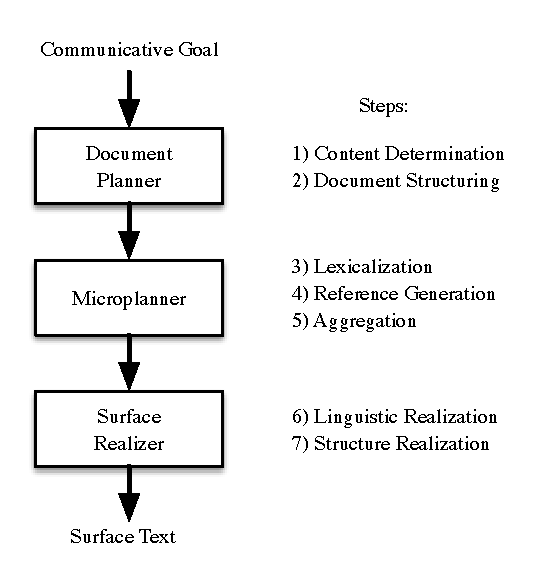
\includegraphics[width=0.69\columnwidth]{Figure/NLG}
\caption{The typical design of a NLG system}
\label{fig:nlg}
\end{figure}

The first main component is the \emph{Document Planner}. The input to this component is a list of features that need to be communicated to
a human reader. By ``content determination'', the document planner interprets the features and creates ``messages''.
After the messages are generated, ``document structuring'' takes place which sorts the messages into a sequence that makes sense to a human reader.

The following component is the \emph{Microplanner}, it decides which words will be used to describe each message. In ``lexicalization'',
the microplanner assigns specific words as parts of speech in a ``phrase'' about each message. Typically, the subject, verb, and object for
a given message are identified. Furthermore, any modifiers such as adjectives and adverbs. Next, two steps aims at smoothing the phrases
so that they are more naturally read, i.e.,  ``Reference generation'' and ``aggregation''.

The last component is the \emph{Surface Realizer}. The surface realizer generates natural language sentences from the phrases.
Different grammar rules for the natural language dictate how the sentences are formed.Then it follows these rules to create
sentences that contain the parts of speech and words given by the microplanner. These sentences are the surface text.


Our \emph{TPD} system processes data generated from Section \ref{modules} as input, following each of the NLG steps shown in Figure \ref{fig:nlg}.

\emph{Content Determination.} In this step, we lock up the activities to be interpreted and extract the context of these activities. For example,
what is the prerequisite activities before certain activity, thus to give hints to developers on reproducing the bugs.

\emph{Document Structuring.} After generating the initial messages in the content determination phase, we put all the messages into
a single document plan. We mainly follow a template based document plan, in which messages occur in a predefined order:
\emph{EventContext, ActionOfEvent}.We decide to use this order as it is natural to read. 

\emph{Lexicalization.} Each type of message needs a specified type of phrase to describe, i.e., in our case, for each type of event
we need to decide on the words to be used to in each of the phrases.
We define a set of phrase templates for each event, some of which are exemplified in Table \ref{tab:eventTemplate}.

\begin{table}[!htbp]
\centering
\small
\caption{Event Template Examples}
\begin{tabular}{|c|} \hline
the user touched the \emph{``Share''} button\\ \hline
the user clicked on the \emph{``Login''} button\\ \hline
the user switched to the \emph{``Content''} interface\\ \hline
the user scrolled down current page\\ \hline
\end{tabular}
\label{tab:eventTemplate}
\end{table}

\emph{Reference Generation and Aggregation.} More complex and readable phrases are generated based on phrases generated
from \emph{Lexicalization} step. The working mechanism of this step is that it looks for patterns of message types, and then groups
the phrases into a sentence. For example, if two messages refer to the same component, then these two phrases of these two
messages are conjoined with and ``and'' and the subject and verb for the second phrase is hidden.  To note, the \emph{Reference Generation}
occurs alongside \emph{Aggregation}.

\emph{Surface Realization.} Finally an external library \emph{simplenlg} \cite{gatt2009simplenlg} is adopted to realize complete sentences from the
phrases formed during \emph{Aggregation}. In the above steps, we set all words and parts of speech and provide the structure of the sentences.
The \emph{simplenlg} follows English grammar rules to concatenate verbs, and make sure the word order, plurals, and articles are correct. 

\subsection{Assemble the Summary}

This part generates the final output of the summary by assembling all the above outcomes, as depicted in the example in Section \ref{intro}.
There are two cases of the summary output, on one hand, the \emph{Decision Model} decides that there are bugs found by the worker.
On the other hand, the \emph{Decision Model} decides no bugs are found by this worker.

For the first case, if there are bugs found by the worker, the final output summary will be constituted of three parts. The first part
is a quick summary that tells the developers there are bugs found for this certain working profile. Then the second part presents
the high risk (potential bugs-related) modules or components that are generated from Section \ref{modules}. Together with the
\emph{TPD} system introduced in Section \ref{tpd}, the key testing processes of the worker are presented as the third part of the
final summary.

While for the second case, it can be very simple,
the summary just tells that there are no bugs found by this working profile.


\section{Evaluation}\label{evaluation}

On the whole, the evaluation of \emph{S-CAT} is binary. That is, both quantitatively and qualitatively.
Mainly, we perform the quantitative evaluation on the part of the \emph{Decision Model}, and the qualitative
evaluation on the final summary.

\subsection{Quantitative Evaluation}

This part of evaluation tests to what extent our \emph{Decision Model} can decide whether bugs are found or not,
based on the working profile. In the ground truth, each working profile is labeled with $1$ if bugs are found, or
$0$ when not.

For the evaluation, we use the metric \emph{Accuracy}, the computation of \emph{Accuracy} proceeds as follows.
We define \emph{hit} for a single test case as either the value $1$ if the class in the test case equals the ground truth, or else
the value $0$. The overall \emph{Accuracy} are defined by averaging all test cases:
\begin{equation}
\small
Accuracy=\frac{\#hit}{|S_{test}|}
\end{equation}
where \emph{\#$hit$} denotes the number of hits in the test set, and $|S_{test}|$ is the number of
all test cases. As we are attempting to evaluate the whole system other than single cases,
this metric well suit our scenario.

\subsection{Qualitative Evaluation}

Two major design goals behind \emph{S-CAT} are: 1) to ease the workload of crowdsourced workers in android testing; 2) facilitate
the developers in debugging. In order to evaluate how effective \emph{S-CAT} is at achieving these goals, we endeavour to evaluate
two major aspects of our framework: 1) \emph{the experience of workers towards the summarization} and 2) \emph{how do the developers
judge the summarization}. As a result, we investigate the following research questions (RQs) as in Table \ref{tab:rq}:

\begin{table}[!h]
\centering
\small
\caption{Research Questions}
\begin{tabular}{c|c} \hline
  \multirow{2}{*}{$RQ_1$} & What information fields are considered as useful\\& that in bug reporting of android testing?\\\hline
  \multirow{2}{*}{$RQ_2$} &Do crowdsourced workers satisfy with the summarization,\\& in volume and in content?\\ \hline
  \multirow{2}{*}{$RQ_3$} &Compared to manually written bug reports,\\& can S-CAT provide sufficient information?\\ \hline
  \multirow{2}{*}{$RQ_4$} &Are summarizations from S-CAT easier to use\\& for deveopers in helping reproduce bugs?\\ \hline
  \multirow{2}{*}{$RQ_5$} &Do developers think the S-CAT provide more hints\\& in debugging than manually written bug reports?\\ \hline
\end{tabular}
\label{tab:rq}
\end{table}

The five RQs were investigated with case studies. And three sets of questions are designed to answer above research questions.
In the following, we will describe the details of the case study.

\emph{Worker Experience.} To assess the worker experience, we ask six different questions in the first study as to answer $RQ_1$ and $RQ_2$,
as listed in Table \ref{tab:qworker}:

\begin{table}[!h]
\centering
\small
\caption{Questions To Assess Worker Experience}
\begin{tabular}{c|c} \hline
$Q_1$ & I thought I would like to use S-CAT frequently.\\ \hline
$Q_2$ &I found S-CAT unnecessary complex.\\ \hline
$Q_3$ & I thought the output of S-CAT was easy to read.\\ \hline
$Q_4$ & I found S-CAT very cumbersome to use.\\ \hline
$Q_5$ & Which part of information do you like most from S-CAT?\\ \hline
$Q_6$ & Which part of information do you like least from S-CAT?\\ \hline
 \end{tabular}
\label{tab:qworker}
\end{table}


The first four questions are answerable as ``Strongly Agree'', ``Agree'', ``Disagree'' or ``Strongly Disagree.'' The last two can be answered as
the ``Decision Part'', ``Potential Modules Part'', ``TPD Part'' or ``None''. The rationale behind these questions is that the output of \emph{S-CAT}
should well express the workers' testing results.


\emph{Developer Experience.} To assess the developer experience, we ask five different questions in the second study as to answer $RQ_4$ and $RQ_5$,
as listed in Table \ref{tab:qdeveloper}:

\begin{table}[!h]
\centering
\small
\caption{Questions To Assess Developer Experience}
\begin{tabular}{c|c} \hline
  \multirow{2}{*}{$Q_7$} & The output of S-CAT contains information\\ & that helps me understand what the bug is.\\\hline
  \multirow{2}{*}{$Q_8$} &The output of S-CAT contains information \\ & that helps me understand where the bug is.\\ \hline
  \multirow{2}{*}{$Q_9$} &The output of S-CAT contains information \\ & that helps me understand how to reproduce the bug.\\ \hline
\end{tabular}
\label{tab:qdeveloper}
\end{table}

Also, the first three questions are answerable as ``Strongly Agree'', ``Agree'', ``Disagree'' or ``Strongly Disagree.''
The rationale behind them is that the summary shall provide enough information to the developers as to help them in debugging.

\emph{Quality of Summary.} And to evaluate the quality of the summary, we ask following six questions in the last study as to answer $RQ_3$,
as listed in Table \ref{tab:quality}.


\begin{table}[!h]
\centering
\small
\caption{Questions To Assess Quality of Summary}
\begin{tabular}{c|c} \hline
  \multirow{2}{*}{$Q_{10}$} &The output of S-CAT covers all the information \\ & compared to the manually-written bug report.\\ \hline
  \multirow{2}{*}{$Q_{11}$} &The output of S-CAT misses important information \\ & compared to the manually-written bug report.\\ \hline
  \multirow{2}{*}{$Q_{12}$} &The output of S-CAT includes information that are \\ & unnecessary compared to the manually-written bug report.\\ \hline
  \multirow{2}{*}{$Q_{13}$} & Independent of other factors, \\ & i feel that the output of S-CAT is accurate.\\ \hline
\end{tabular}
\label{tab:quality}
\end{table}

Each of these four multiple choice questions could be answered as ``Strongly Agree'', ``Agree'', ``Disagree'' or ``Strongly Disagree.''
And the rationale behind these four questions is that the summary shall be accurate in deciding which information to present
while not being too cumbersome.

We assigned values to these answers as $4$ for ``Strongly Agree'', $3$ for ``Agree'', $2$ for ``Disagree'' and $1$ for ``Strongly Disagree.''
For questions $1,3,7,8,9,10$ and $13$, higher values indicate stronger performance. While for questions $2,4,11$ and $12$, lower values are preferred.
The responses to each questions are then aggregated.


\section{Experiment}\label{exp}

This section reports the results of our evaluation. First, we describe the data we are using for the experiments, and then we present
the results, along with our interpretation.

\subsection{Data}
We conducted our experiments with data from our crowdsourced android testing platform, i.e., Kikbug\footnote{http://kikbug.net}.
Specifically, testing data of three applications are used to evaluate the performance of \emph{S-CAT}, which are \texttt{SE-1800}, \texttt{UBook} and \texttt{iShopping}.
\texttt{SE-1800} is an electrical monitoring application, and \texttt{UBook} is an online education application and \texttt{iShopping} is an online shopping guide application.
All the three crowdsourced testing tasks were performed between the time period $October, 2015$ and $January, 2016$. In the implementation,
all the information mentioned in Section \ref{problemDef} were collected through the android client and reported by the crowdsourced workers, i.e., the screenshots,
the logcat file and event sequence, as well as a manually-written report. After the finish of the tasks, all the reports were validated by the
developers of the applications, each was labelled as bugs found or not. Statistical information about the data we are using are illustrated
in Table \ref{tab:stats}, in which we present the number of workers taking that specific testing task, the valid report means the the manually-written
report that is confirmed by the developer, and the validated bug means the worker reports a bug which is validated by the developer,
the valid working profile mainly concerns about whether the logcat file and event sequence are successfully collected or not.

\begin{table}[h]
\centering
\small
\caption{Statistics of The Data}
\begin{tabular}{cccc}
\hline
App & \texttt{SE-1800} & \texttt{UBook} & \texttt{iShopping} \\ \hline
\#Workers & $132$ & $142$ & $173$ \\ \hline
\#Valid Report & $109$ & $125$ & $147$ \\ \hline
\#Validated Bug & $55$ & $63$ & $78$ \\ \hline
\#Valid Working Profile & $101$ & $105$ & $122$ \\ \hline
\end{tabular}
\label{tab:stats}
\end{table}


\subsection{Participants}

We had $19$ participants in our case study. Fifteen were graduate students with background of Computer Science and Engineering, the remaining
four were professional programmers from two different organizations, not listed due to our privacy policy. Each participant was required to review
$9$ summaries, we randomly chose three \emph{S-CAT} outputs from each of the three applications. And based on the summaries, the
$13$ questions were answered in order to answer the aforementioned research questions. Of the $19$ participants, $2$ did not
complete enough of the study, whom were graduate students, and their results are thrown out.

\subsection{Results and Discussion}

\subsubsection{Quantitative Results}

We first report the results of the accuracy of the \emph{Decision Model} in deciding whether bugs are found or not.
In the experiment, we adopted the $10$-fold cross validation to train and test the classifier, as the amount of available
data in our experiment is limited. And the mean average accuracy is presented in Table \ref{tab:acc}. On average,
the \emph{Decision Model} can achieve an accuracy around $0.9$ on all the three applications.

\begin{table}[h]
\centering
\small
\caption{Average Accuracy}
\begin{tabular}{cccc}
\hline
App & \texttt{SE-1800} & \texttt{UBook} & \texttt{iShopping} \\ \hline
Accuracy & $0.8935$ & $0.9167$ & $0.9013$ \\ \hline
\end{tabular}
\label{tab:acc}
\end{table}

Currently, the realization of the \emph{Decision Model} simply picks out some naive features that are related to the finding
of bug, and adopts the SVM to train a classifier. We don't claim the improvement of the accuracy of this component as our contribution,
and our framework is extensible as new classification models and new features can be imported to fulfil the task as deciding
whether bugs are found or not in this step of the \emph{S-CAT}.

\subsubsection{Qualitative Results}

Figure \ref{fig:high}, Figure \ref{fig:low} and Figure \ref{fig:open} summarize the results of our case study.
The box-plots in Figure \ref{fig:high} and Figure \ref{fig:low} illustrates the aggregated responses of users to
questions that can be answered as as ``Strongly Agree'', ``Agree'', ``Disagree'' or ``Strongly Disagree.''
And Figure \ref{fig:open} present the aggregated answers to which part of the \emph{S-CAT} they like most/least, in
which ``DM'' means the \emph{Decision Model}, ``HRM'' means the component of high risk modules or say potential bugs-related modules,
and ``TPD'' means the \emph{TPD} module. In particular, the figures depict the answers to questions when higher values indicate stronger performance (Figure \ref{fig:high}),
the answers to those questions when lower values are preferred (Figure \ref{fig:low}), as well as the answers to questions
when certain components of the framework shall be indicated (Figure \ref{fig:open}).

In regard to the worker experience, we explore the results to questions $1, 2, 3, 4, 5$ and $6$. From the user responses,
we can tell that: 1) the users have a high tendency to use \emph{S-CAT} ($Q_1$), 2) mostly, the users thought the \emph{S-CAT}
is intuitive and very easy to understand ($Q_2$, $Q_4$), and the output is easy to read ($Q_3$), 3) though some may not
like parts of the \emph{S-CAT} ($Q_6$ in Figure \ref{fig:open}), most of the users ($16$ of $17$) expressed their favours on
certain parts of the framework ($Q_6$), and among the three components, the users liked the ``TPD'' the most ($8$).
Based on these results we can answer $\emph{RQ}_1$ and $\emph{RQ}_2$ as follows:
\emph{The users are satisfied with the output of \emph{S-CAT}, in both readability and usefulness.}


\begin{figure}[!htbp]
\centering
\includegraphics[width=0.63\columnwidth]{Figure/highanswer}
\caption{Q$1, 3, 7, 8, 9, 10$ and $13$}
\label{fig:high}
\end{figure}

\begin{figure}[!htbp]
\centering
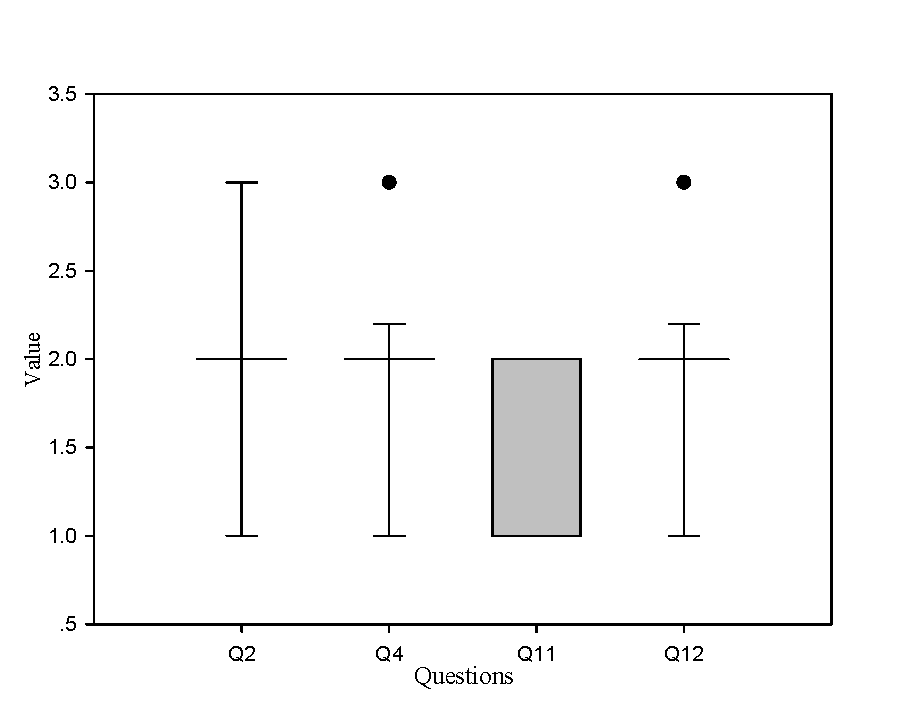
\includegraphics[width=0.63\columnwidth]{Figure/lowanswer}
\caption{Q$2, 4, 11$ and $12$}
\label{fig:low}
\end{figure}


\begin{figure}[!htbp]
\centering
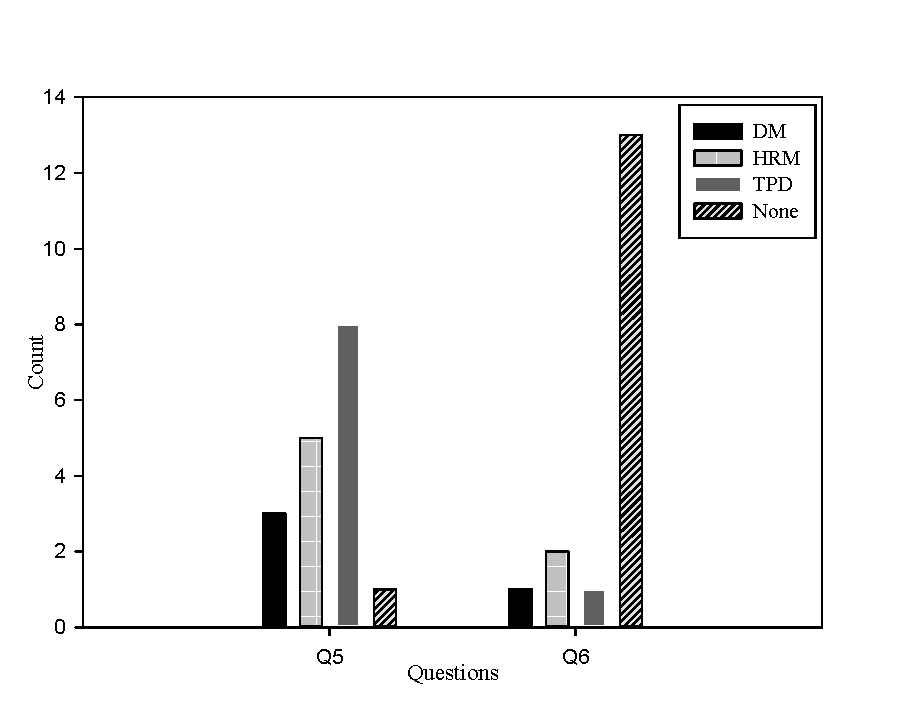
\includegraphics[width=0.63\columnwidth]{Figure/openanswer}
\caption{Answers to question $5$ and $6$}
\label{fig:open}
\end{figure}


Regarding the developer experience, we exploit the answers to questions $7, 8$ and $9$.
From the user responses, we can tell that: 1) most users agree in that the generated summary helps in
understanding what the bug is ($Q_7$), 2) and they also hold the opinion the summary from \emph{S-CAT}
provides information in deciding where the bug is ($Q_8$), 3) as well as hints on how to reproduce a
certain bug from the component of \emph{TPD} ($Q_9$).
Therefore, we can answer $\emph{RQ}_4$ and $\emph{RQ}_5$ as follows:
\emph{The users have a strong belief that the \emph{S-CAT} can well facilitate the developers
in understanding the bugs and locating the bugs, as well as reproducing the bugs.}

In terms of the quality of summary, we refer to the answers to questions $10, 11, 12$ and $13$.
From the responses of users, we can easily get the following conclusions: 1) mostly, the information \emph{S-CAT}
provided can cover all the information compared to the manually-written report by the crowdsourced worker ($Q_{10}$),
2) and it covers all the important information, while not to be cumbersome ($Q_{11}$,$Q_{12}$), 3) the users also
agreed on that the information \emph{S-CAT} conveyed is accurate for both the deciding of potential bugs-related modules
and the description for key testing processes.
Thus, we can answer $\emph{RQ}_3$ as follows:
\emph{The users are satisfied with the quality of output from \emph{S-CAT}, in terms of coverage and accuracy.}


\section{Related Work}\label{relatedwork}

There are three lines of work we would like to address as the related work, i.e., \emph{Crowdsourced Testing}, \emph{Summarization} and \emph{Android Testing}.

\emph{Crowdsourcing Testing}. Crowdsourcing arose with citizen science as a form of volunteerism, but now spans the gamut from work (paid microtasking)
to play (games for good) \cite{michelucci2016power}. Typically, crowdsourcing outsources a job to an undefined, generally large group of people
in the form of an open call, which is conventionally performed by a designated agent (usually an employee) \cite{difallah2015dynamics,estelles2012towards,conf/icse/MaoYLH04}.
Along with this trend, crowdsourced testing is gaining more and more attention from industry.
Liu et al. \cite{liu2012crowdsourcing} applied crowdsourced testing in the usability testing. They studied both methodological differences for crowdsourcing usability testing and
empirical contrasts to results from more traditional, face-to-face usability testing. 
Dolstra  et al. \cite{icst/DolstraVP13} used crowdsourced testing to perform the expensive tasks on GUI testing. They use virtual machines to run
the system under test and enable semi-automated GUI testing by crowdsourced workers. Nebeling et al. \cite{nebeling2012crowdsourced} evaluated
the usability of web sites and web-based services with crowdsourcing data, where they showed that crowdsourcing data could provide an efficient
and effective testing method to the web interfaces.

\emph{Summarization}. Summarization has been successfully applied to many domains like news articles \cite{radev2001newsinessence}, social media \cite{lin2009summarization},
medical documents \cite{afantenos2005summarization}, videos \cite{han2011personalized}, audio \cite{waibel2001advances} and trajectory \cite{su2015making},
in addition to technical documents. The related works closest to our approach is summarizing bug reports, which have been previous studied in \cite{rastkar2010summarizing}, in which they used
supervised methods to automatically generate one kind of software artifact, bug reports, to provide developers with the benefits others experience daily in other
domains. Then, Mani et al. \cite{mani2012ausum} studied unsupervised summarization techniques for bug summarization, the efficacy of their unsupervised techniques
were improved by applying noise identifier and filtering methods. There are also a number of other approaches studying summarizing different software artifacts and behaviors.
Sridhara et al. developed novel heuristics to automatically summarize a Java method in the form of natural language comments \cite{sridhara2010towards}. Moreno et al. \cite{haiduc2010use} proposed a summarization
technique for Java classes that match one of $13$ ``stereotypes''. Specifically, their technique selects statements from the class based on this stereotype, and then
uses the approach by Sridhara \cite{sridhara2010towards} to summarize those statements. A most recent work by McBurney and McMillan \cite{mcburney2015automatic}
summarized the context of the source code, such as how the code is called or the output is used.

\emph{Android Testing}. Besides the traditional failures due to application logic bugs, android applications often show failures that are specific of their development platform,
mobile context, connectivity and so on so forth. Some specific android bugs are reported in the classification proposed by Hu et al. \cite{hu2011automating},
as well as an android-specific testing technique, which is event-based and focuses on \emph{Activity}, \emph{Event} and dynamic type errors. Android
testing has also been approached by model-based testing techniques. Takala et al. \cite{takala2011experiences} described a model-based approach
for android GUI testing, their technique described the GUI of an android application by state machines. An alternative approach for automatically testing
an android application by its GUI was proposed by Amalfitano et al. \cite{amalfitano2011gui}, whose approach was based on a tool that explores the application
GUI by simulating real user events on the user interface and reconstructs a GUI tree model. Our approach differs in that the \emph{S-CAT} deals with crowdsourced testing,
where the mobile contexts, device hardwares and system version releases are diversified.



\section{Conclusions}\label{conclusions}


Crowdsourcing is an ideal solution to the android testing due to all the portability and compatibility issues. However, it meets the problem of quality control.
There are two major sets of approaches that aim at the quality control in it, i.e., the design-time approaches, e.g.,
effective task preparation and worker selection, and the other is runtime approaches, e.g., expert review, ground truth, majority consensus, contributor evaluation,
real-time support and workflow management.
In this paper, we have proposed a framework \emph{S-CAT} to summarize the crowdsourced android testing, as an answer to the problem of
quality control in the specified crowdsourcing circumstance, i.e., android testing, by adopting the idea of real-time support. Our pilot evaluation results demonstrated
the proposed \emph{S-CAT} is effective in both easing the workload of workers and facilitating the developers in debugging.




% An example of a floating figure using the graphicx package.
% Note that \label must occur AFTER (or within) \caption.
% For figures, \caption should occur after the \includegraphics.
% Note that IEEEtran v1.7 and later has special internal code that
% is designed to preserve the operation of \label within \caption
% even when the captionsoff option is in effect. However, because
% of issues like this, it may be the safest practice to put all your
% \label just after \caption rather than within \caption{}.
%
% Reminder: the "draftcls" or "draftclsnofoot", not "draft", class
% option should be used if it is desired that the figures are to be
% displayed while in draft mode.
%
%\begin{figure}[!t]
%\centering
%\includegraphics[width=2.5in]{myfigure}
% where an .eps filename suffix will be assumed under latex, 
% and a .pdf suffix will be assumed for pdflatex; or what has been declared
% via \DeclareGraphicsExtensions.
%\caption{Simulation results for the network.}
%\label{fig_sim}
%\end{figure}

% Note that the IEEE typically puts floats only at the top, even when this
% results in a large percentage of a column being occupied by floats.


% An example of a double column floating figure using two subfigures.
% (The subfig.sty package must be loaded for this to work.)
% The subfigure \label commands are set within each subfloat command,
% and the \label for the overall figure must come after \caption.
% \hfil is used as a separator to get equal spacing.
% Watch out that the combined width of all the subfigures on a 
% line do not exceed the text width or a line break will occur.
%
%\begin{figure*}[!t]
%\centering
%\subfloat[Case I]{\includegraphics[width=2.5in]{box}%
%\label{fig_first_case}}
%\hfil
%\subfloat[Case II]{\includegraphics[width=2.5in]{box}%
%\label{fig_second_case}}
%\caption{Simulation results for the network.}
%\label{fig_sim}
%\end{figure*}
%
% Note that often IEEE papers with subfigures do not employ subfigure
% captions (using the optional argument to \subfloat[]), but instead will
% reference/describe all of them (a), (b), etc., within the main caption.
% Be aware that for subfig.sty to generate the (a), (b), etc., subfigure
% labels, the optional argument to \subfloat must be present. If a
% subcaption is not desired, just leave its contents blank,
% e.g., \subfloat[].


% An example of a floating table. Note that, for IEEE style tables, the
% \caption command should come BEFORE the table and, given that table
% captions serve much like titles, are usually capitalized except for words
% such as a, an, and, as, at, but, by, for, in, nor, of, on, or, the, to
% and up, which are usually not capitalized unless they are the first or
% last word of the caption. Table text will default to \footnotesize as
% the IEEE normally uses this smaller font for tables.
% The \label must come after \caption as always.
%
%\begin{table}[!t]
%% increase table row spacing, adjust to taste
%\renewcommand{\arraystretch}{1.3}
% if using array.sty, it might be a good idea to tweak the value of
% \extrarowheight as needed to properly center the text within the cells
%\caption{An Example of a Table}
%\label{table_example}
%\centering
%% Some packages, such as MDW tools, offer better commands for making tables
%% than the plain LaTeX2e tabular which is used here.
%\begin{tabular}{|c||c|}
%\hline
%One & Two\\
%\hline
%Three & Four\\
%\hline
%\end{tabular}
%\end{table}


% Note that the IEEE does not put floats in the very first column
% - or typically anywhere on the first page for that matter. Also,
% in-text middle ("here") positioning is typically not used, but it
% is allowed and encouraged for Computer Society conferences (but
% not Computer Society journals). Most IEEE journals/conferences use
% top floats exclusively. 
% Note that, LaTeX2e, unlike IEEE journals/conferences, places
% footnotes above bottom floats. This can be corrected via the
% \fnbelowfloat command of the stfloats package.



% conference papers do not normally have an appendix


% use section* for acknowledgment



% trigger a \newpage just before the given reference
% number - used to balance the columns on the last page
% adjust value as needed - may need to be readjusted if
% the document is modified later
%\IEEEtriggeratref{8}
% The "triggered" command can be changed if desired:
%\IEEEtriggercmd{\enlargethispage{-5in}}

% references section

% can use a bibliography generated by BibTeX as a .bbl file
% BibTeX documentation can be easily obtained at:
% http://mirror.ctan.org/biblio/bibtex/contrib/doc/
% The IEEEtran BibTeX style support page is at:
% http://www.michaelshell.org/tex/ieeetran/bibtex/
%\bibliographystyle{IEEEtran}
% argument is your BibTeX string definitions and bibliography database(s)
%\bibliography{IEEEabrv,../bib/paper}
%
% <OR> manually copy in the resultant .bbl file
% set second argument of \begin to the number of references
% (used to reserve space for the reference number labels box)


\bibliographystyle{abbrv}
\bibliography{sigproc}




% that's all folks
\end{document}


